\begin{figure}
    \begin{center}
    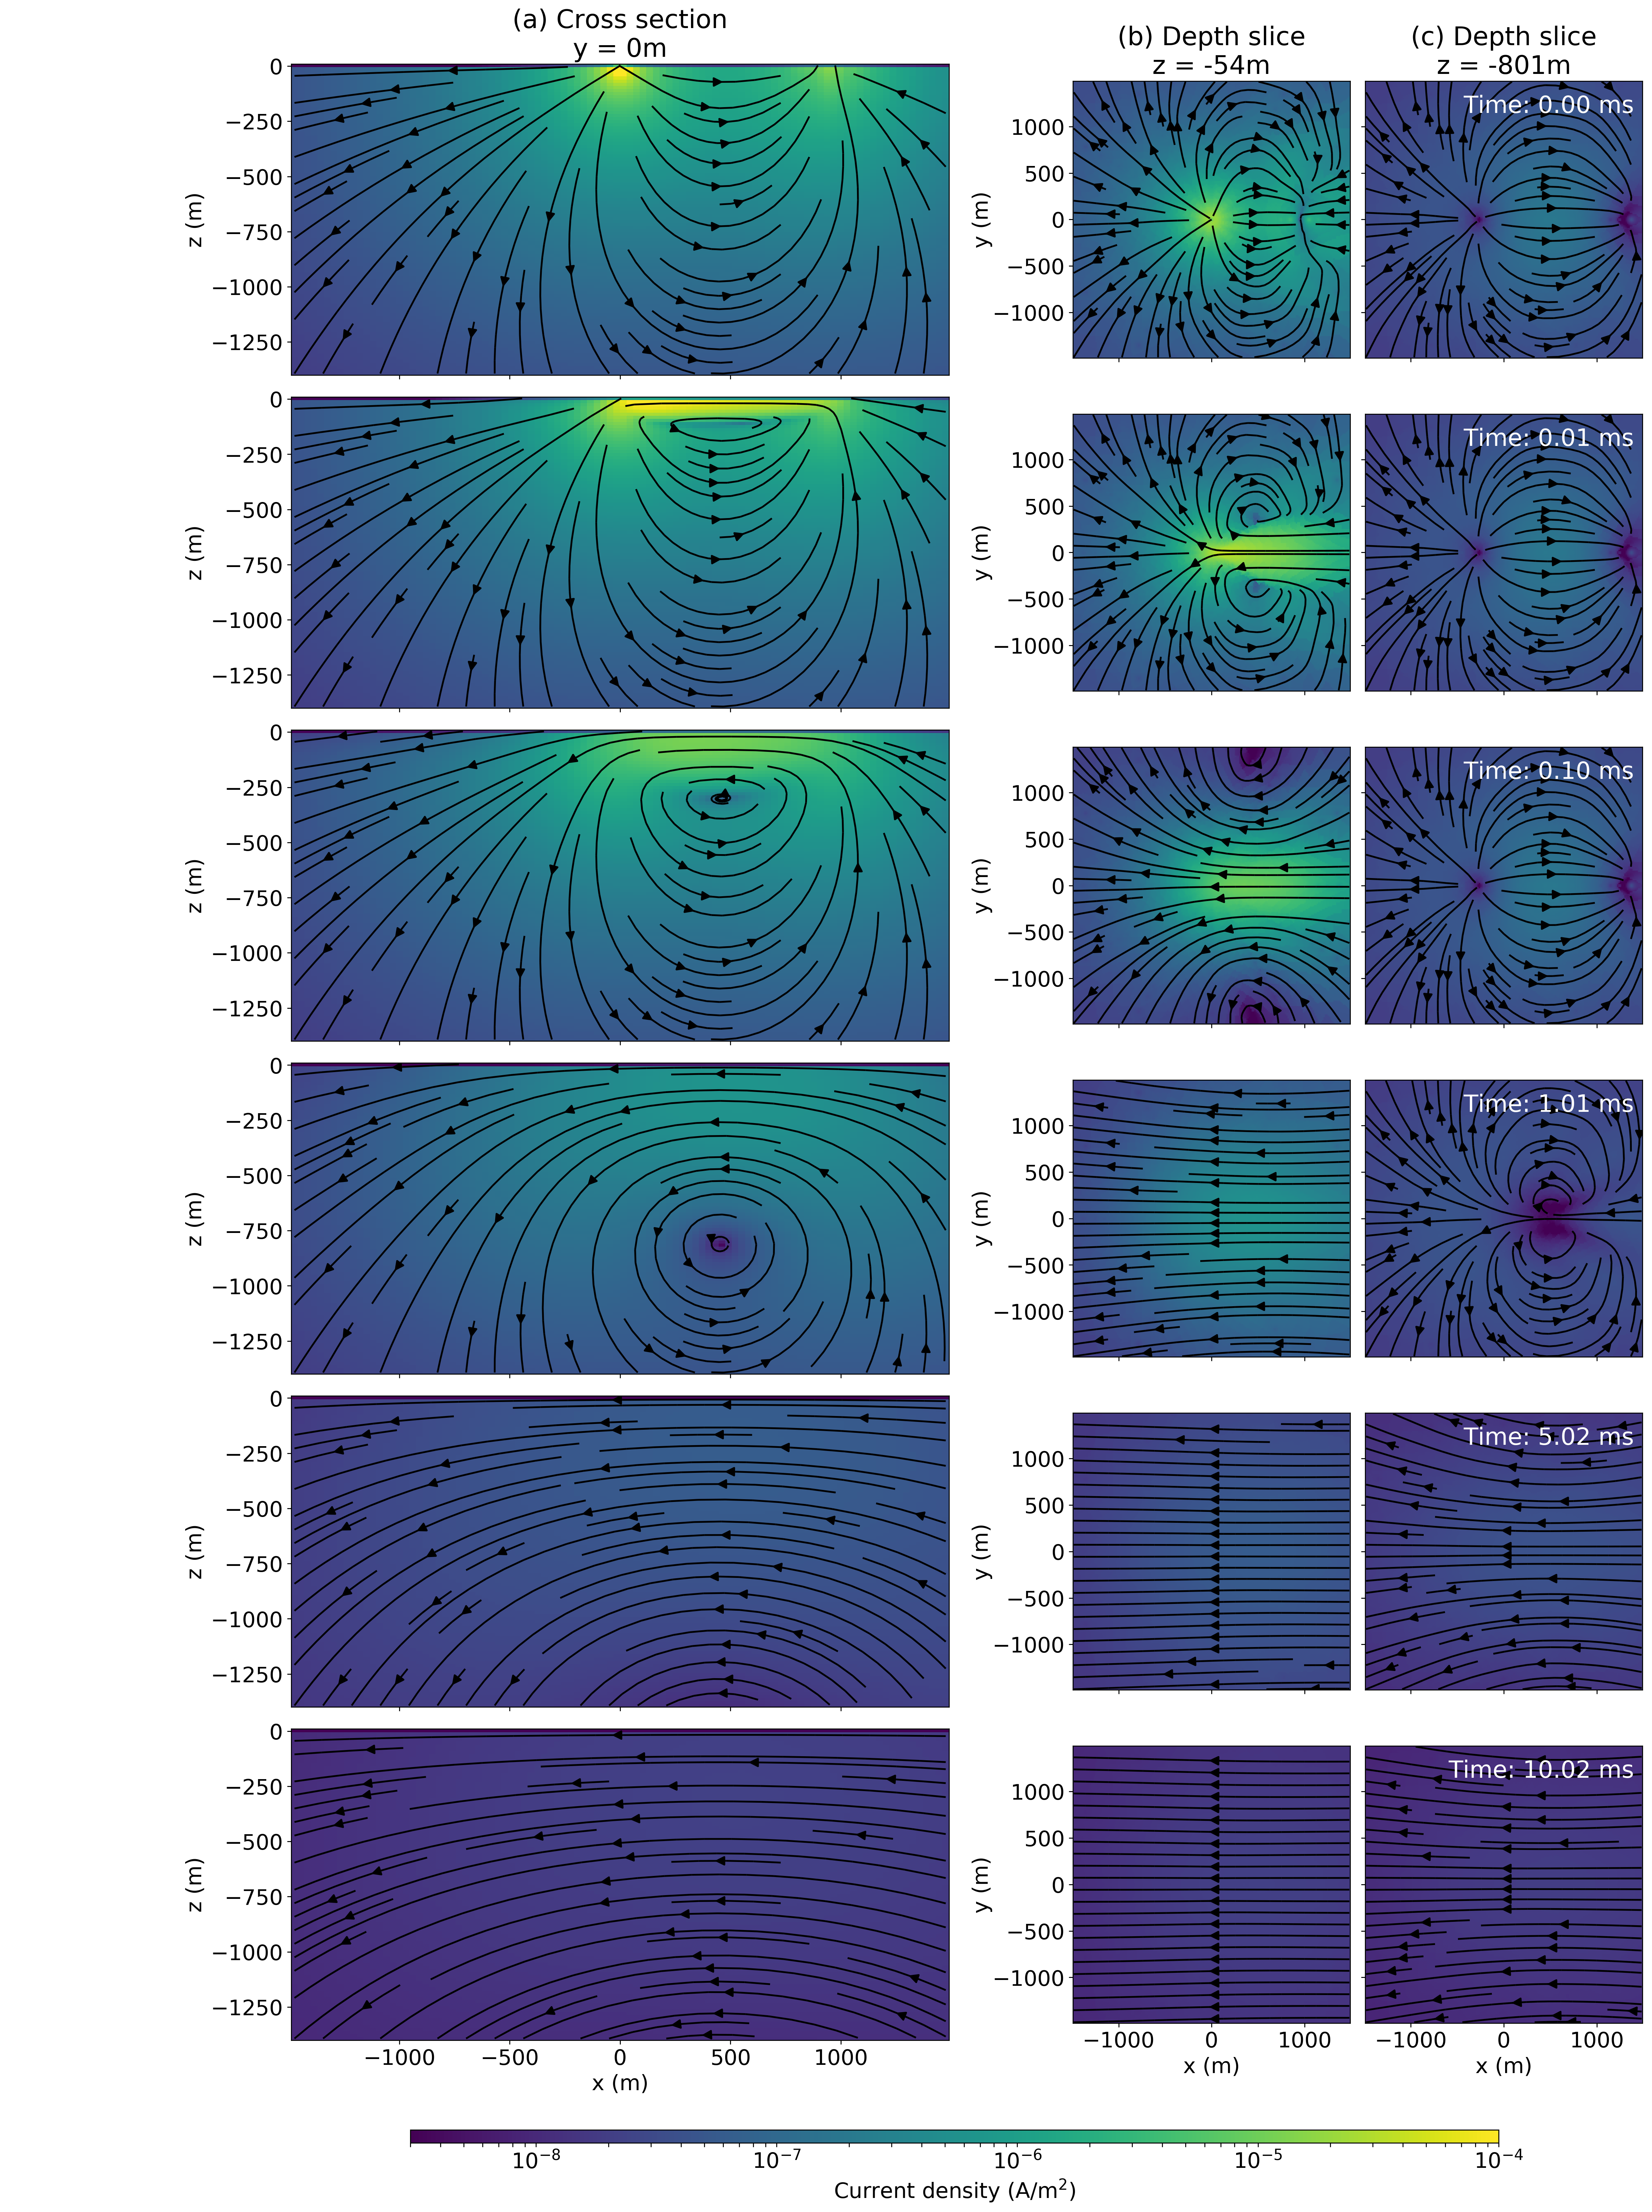
\includegraphics[width=0.85\textwidth]{figures/em_casing/tdem-background-total-currents.png}
    \end{center}
\caption{
    Current density for a time domain experiment over a $10^{-2}$ S/m half-space.
    The positive electrode is on the surface where the well-head will be and the return electrode is at $x=1000$ m. Each row corresponds to different time, as indicated in the plots in panel (c). Panel (a) shows a cross section through the half-space along the same line as the source-wire. Panels (b) and (c) show depth-slices of the currents at 54 m and 801 m depth.
}
\label{fig:tdem-background-total-currents}
\end{figure}



